The Cellular Automata Research Platform has been the subject of three previous master theses at NTNU.
The original implementation was made by Djupdal in 2003.
It was then extended with a range of various output methods by Aamodt in 2005.
Finally, it was further extended and optimized in expectation of new hardware by Støvneng in 2014.

\subsection{Conception}

In 2002, NTNU invested in a CompactPCI computer with a NallaTech BenERA FPGA board to be used for research within the field of evolutionary hardware.
The task of developing a platform for the system, based on a matrix of sblocks, fell to Djupdal \cite{djupdal2003sblock}.

An overview of the resulting hardware platform is shown in \figurename~\ref{fig:overview-djupdal}.
It consists of the mentioned sblock matrix, BRAM for storing the state and type of each cell, a development unit, control logic, and a PCI communication unit.

\begin{figure}[!ht]
    \centering
    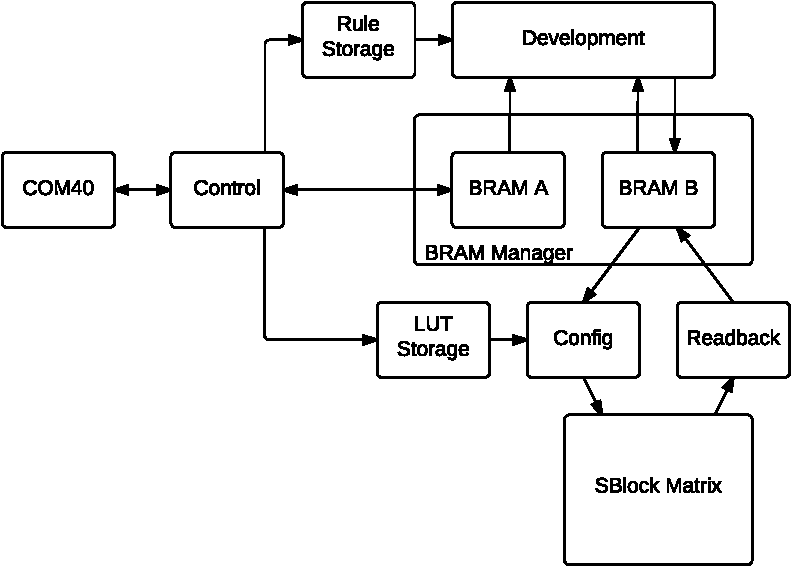
\includegraphics[width=0.48\textwidth]{figures/overview-djupdal}
    \caption{High-level block diagram of hardware platform after Djupdal's original work.}
    \label{fig:overview-djupdal}
\end{figure}

\subsection{Extension: Aamodt \cite{aamodt2005sblock}}

\begin{itemize}
    \item Fig. \ref{fig:overview-aamodt}
\end{itemize}

\begin{figure}[!ht]
    \centering
    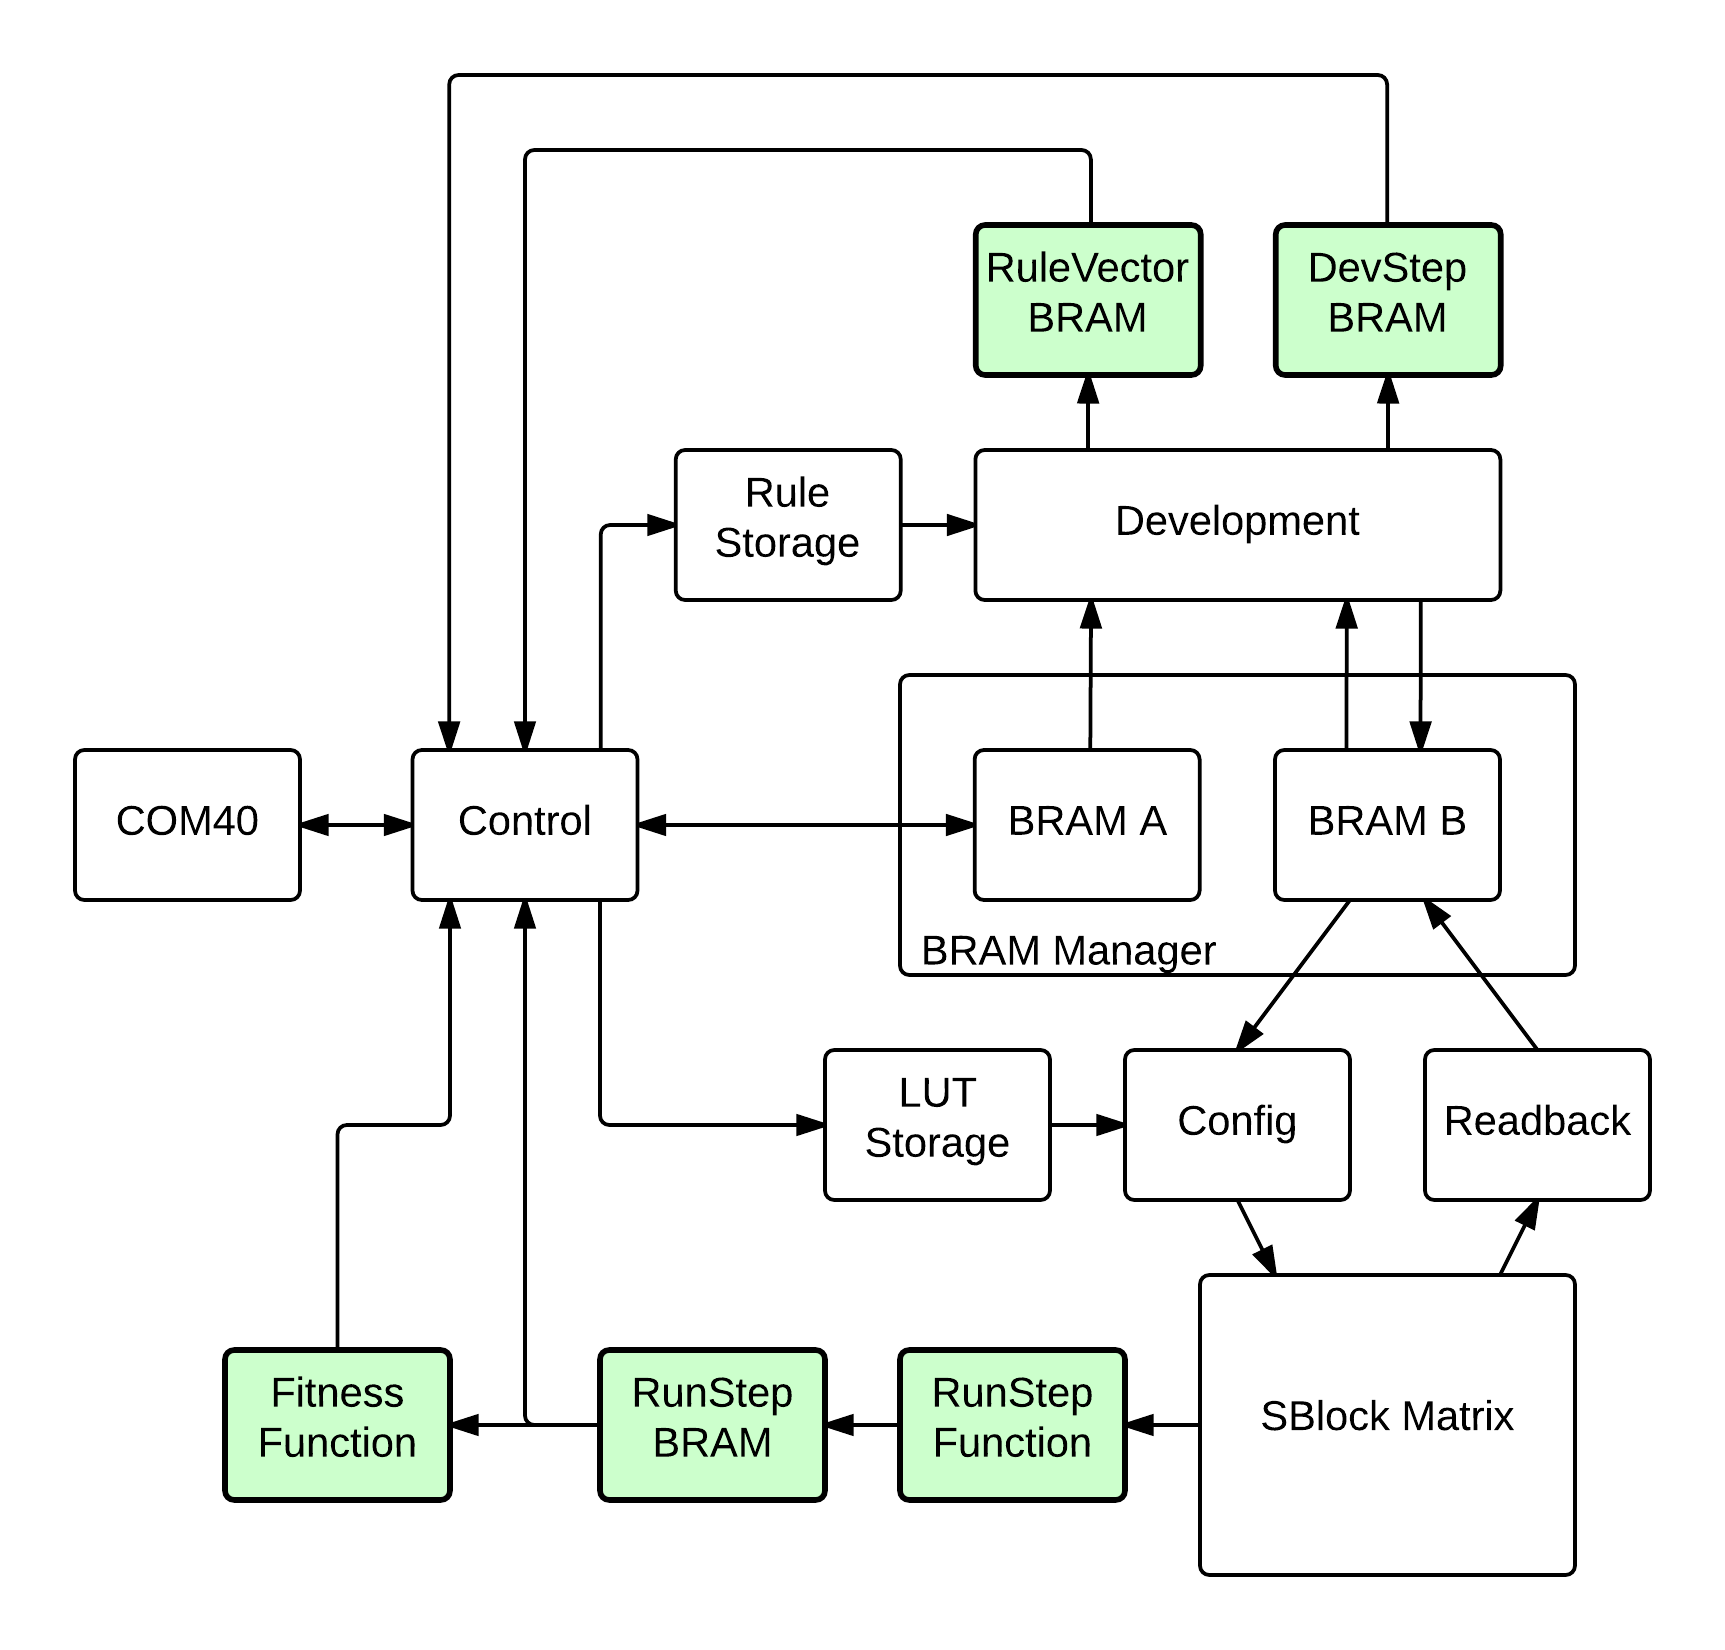
\includegraphics[width=0.48\textwidth]{figures/overview-aamodt}
    \caption{Aamodt's additions in green}
    \label{fig:overview-aamodt}
\end{figure}

\subsection{Renovation: Støvneng \cite{stovneng2014sblock}}

\begin{itemize}
    \item New hardware
    \item Fig. \ref{fig:overview-stovneng}
\end{itemize}

\begin{figure}[!ht]
    \centering
    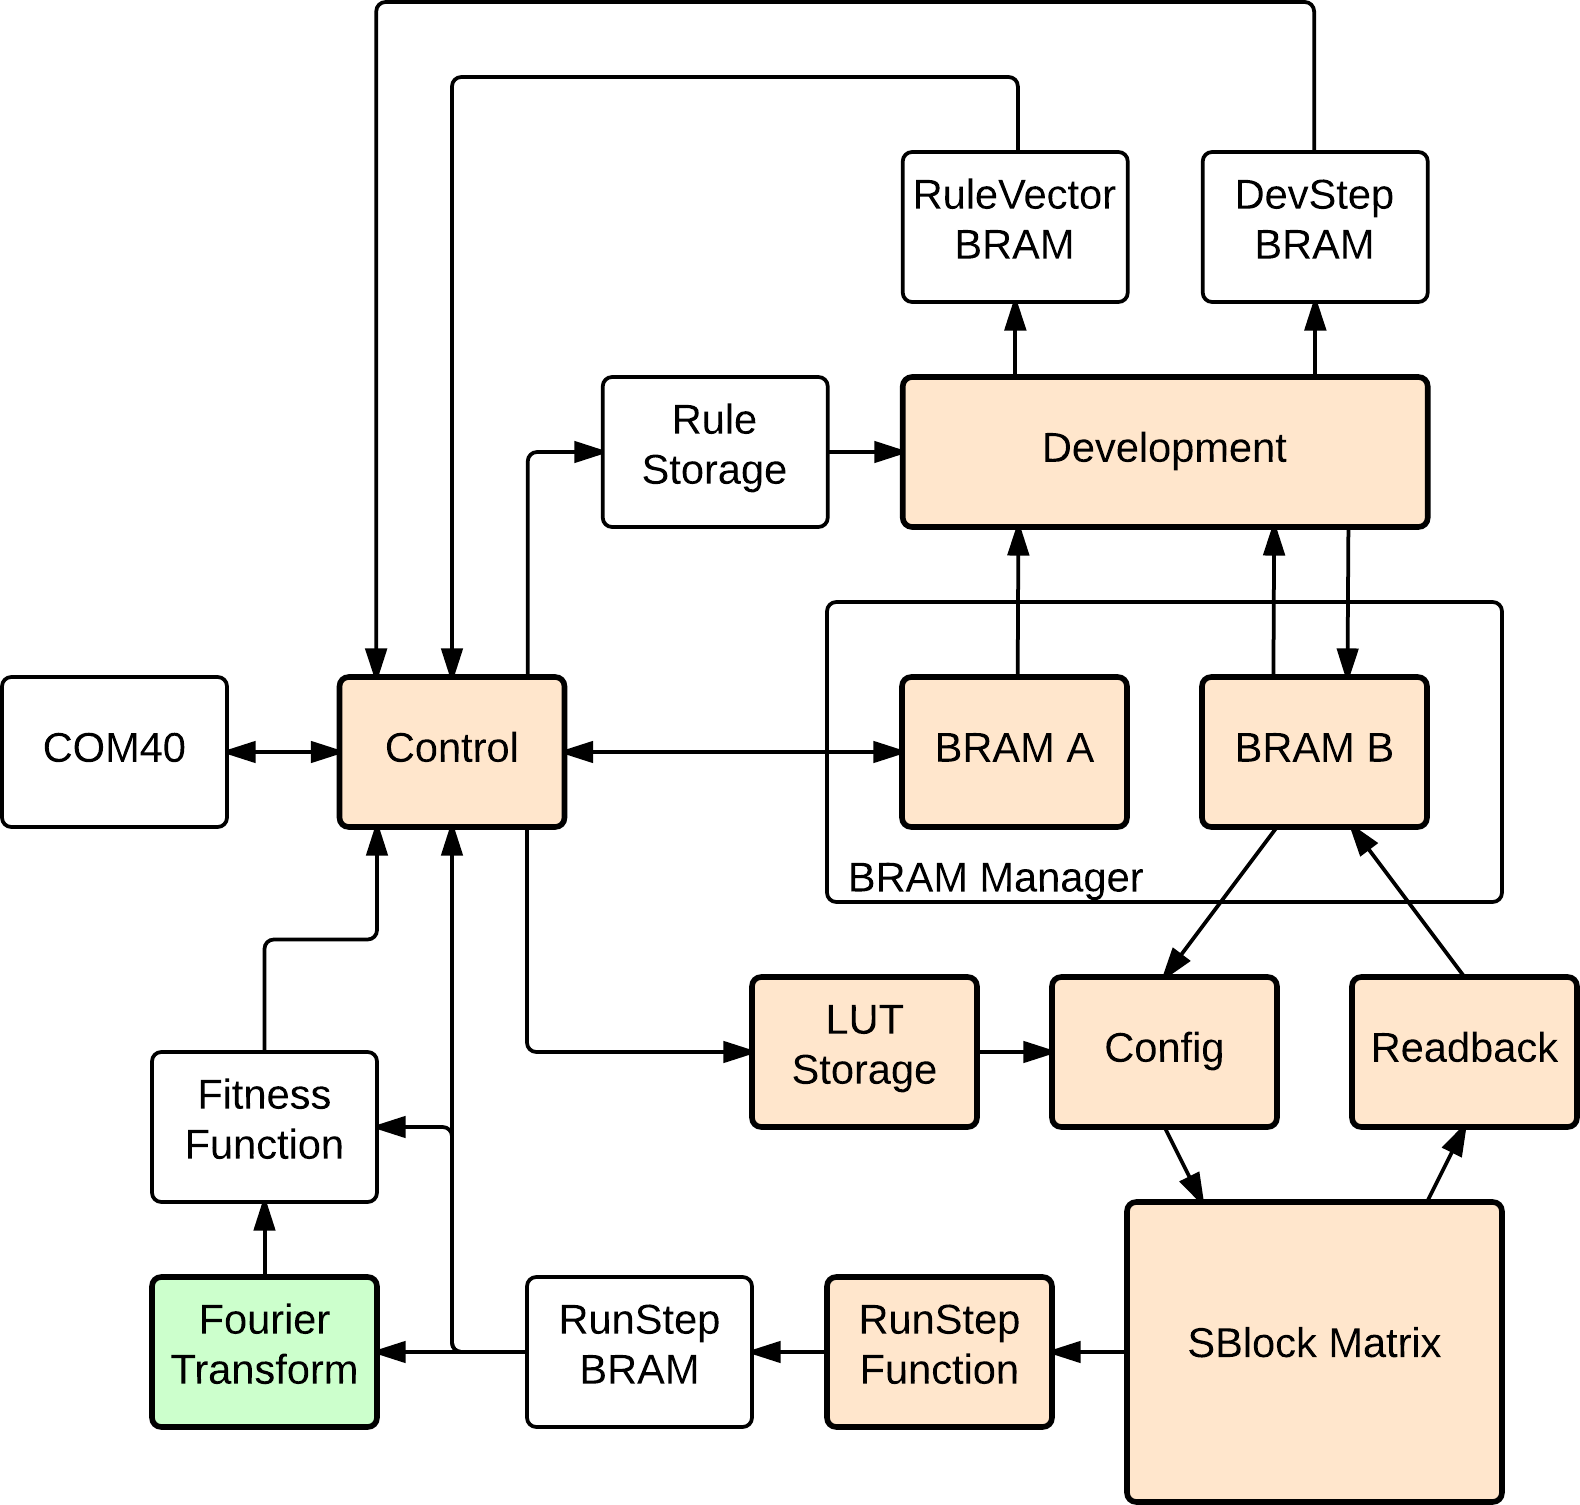
\includegraphics[width=0.48\textwidth]{figures/overview-stovneng}
    \caption{Støvneng's additions in green, optimizations and/or 3D modifications in orange}
    \label{fig:overview-stovneng}
\end{figure}

